\section{Case Study} \label{sec:case}


\subsection{Experimental Setup}

\begin{table}[t]
\centering
\caption{Simulation Parameters}
\label{tb:parameters}
\vspace{-5pt}
\begin{tabular}{ l | c }
\hline \hline
Components & Features\\
\hline
Simulator kernel & SystemC 2.2.0\\
\hline
CPU core & ARM9TDMI and XScale compatible \\
\hline
\multirow{2}{*}{Cache configurations} & 4-way associative 16K L1 cache  \\
& 4B cache line size \\
\hline
\multirow{2}{*}{Bus} & 32-bit address bus  \\
& 32-bit data bus \\
\hline
Clock frequency & $1GHz$ \\
\hline
Main memory & 64MB DRAM \\
\hline
Benchmark & MiBench \\
\hline\hline
\end{tabular}
\vspace{-10pt}
\end{table}

\subsection{Experimental Results}

\begin{figure}[t]
\centering
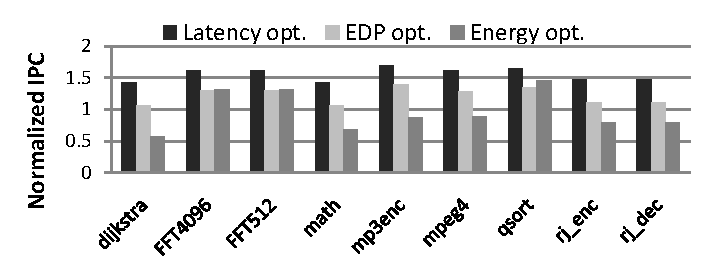
\includegraphics[width=0.4\textwidth]{fig/IPC}
\vspace{-10pt}
\caption{Normalized IPC for STT-RAM with different optimization directions.}
\label{fig:pic}
\vspace{7pt}
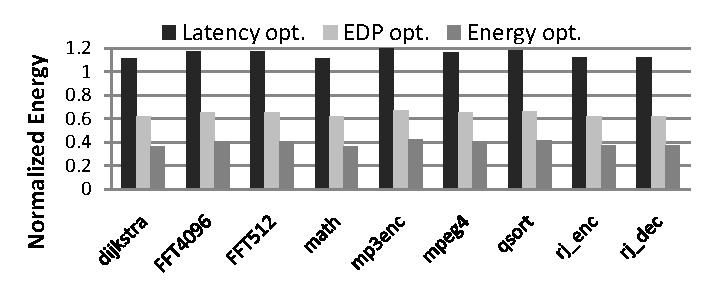
\includegraphics[width=0.4\textwidth]{fig/Energy}
\vspace{-10pt}
\caption{Normalized energy for STT-RAM with different optimization directions.}
\label{fig:energy}
\vspace{7pt}
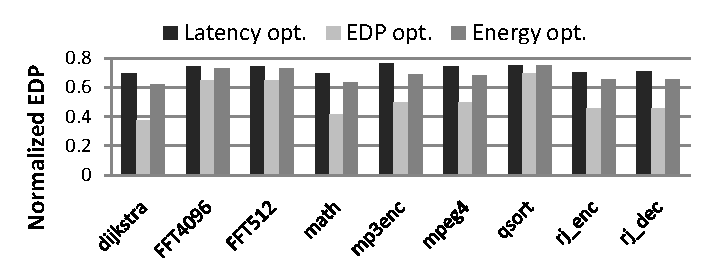
\includegraphics[width=0.4\textwidth]{fig/EDP}
\vspace{-10pt}
\caption{Normalized EDP for STT-RAM with different optimization directions.}
\label{fig:edp}
\vspace{-10pt}
\end{figure} 

\begin{figure}[t]
  \centering
  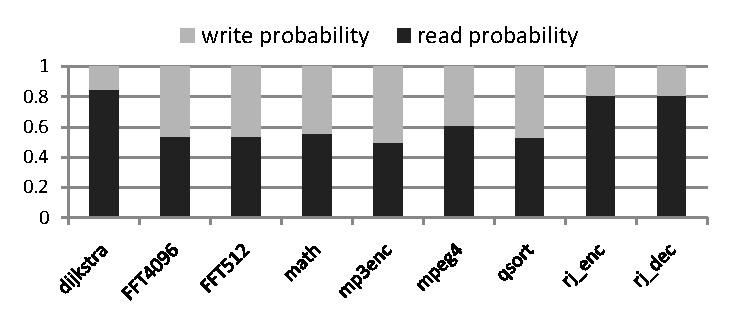
\includegraphics[width=2.8in]{fig/RWratio.eps}
  \vspace{-10pt}
  \caption{Read-write ratio for different benchmarks.}
  \label{fig:ratio}
\vspace{-15pt}
\end{figure}